% Plantilla para los PICs 
% Version 0.1
% 02/06/2022
% Por: pfordonez@unl.edu.ec 


% Elige si deseas optimizar la ejecución del proyecto almacenando las figuras generadas con TikZ y PGF en una carpeta (archivos/figuras-procesadas).
% 1 - Si, 2 - No
\def\OptimizaTikZ{2}
%%%%%%%%%%%%%%%%%%%%%%%%%%%%%%%%%%%%%%%%%%%%%%%%%%%%%%%%%%%%%%%%%%%%%%%%
% Plantilla TFG/TFM
% Realizado por: Jose Manuel Requena Plens
% Contacto: info@jmrplens.com / Telegram:@jmrplens
%%%%%%%%%%%%%%%%%%%%%%%%%%%%%%%%%%%%%%%%%%%%%%%%%%%%%%%%%%%%%%%%%%%%%%%%

%%%%%%%%%%%%%%%%%%%%%%%%
% FORMATO DEL DOCUMENTO
%%%%%%%%%%%%%%%%%%%%%%%%
% scrbook es la clase de documento
% Si se desea que no haya página en blanco entre capítulos añadir "openany" en los parámetros de la clase. Sino siempre los capítulos empezarán en página impar.
\documentclass[a4paper,12pt,titlepage,openany]{scrbook}
\KOMAoption{toc}{bib,chapterentryfill} % Opciones del índice
\usepackage{scrhack} % Previene algunos errores
% Paquete de formato para scrbook. Con marcas, linea-separador superior e inferior
\usepackage[automark,headsepline,footsepline]{scrlayer-scrpage}
\clearpairofpagestyles		% Borra los estilos por defecto
%%
% Formato y contenido de la información de cabecera y pie de página
%%
% Información de capítulo en cabecera e interno
\ihead{{\color{gray30}\scshape\small\headmark}}	
% Número de página en cabecera y externo
\ohead{\normalfont\pagemark} 
% Número de página en pie de página y externo. Sólo en páginas sin cabecera
\ofoot[\normalfont\pagemark]{}
%% 		
% Edición del contenido de las distintas partes de la cabecera
%%
\renewcommand{\chaptermark}[1]{\markboth{#1}{}} % Capítulo (Solo texto)
\renewcommand{\sectionmark}[1]{\markright{\thesection. #1}} % Sección (Número y texto)
\setkomafont{pagenumber}{} % Número de página (Sin nada añadido)

% Añade al índice y numera hasta la profundidad 4.
% 1:section,2:subsection,3:subsubsection,4:paragraph
\setcounter{tocdepth}{4}
\setcounter{secnumdepth}{4}
% Muestra una regla para comprobar el formato de las páginas
%\usepackage[type=upperleft,showframe,marklength=8mm]{fgruler}
% MÁRGENES DE LAS PÁGINAS
\usepackage[
  inner	=	3.0cm, % Margen interior
  outer	=	2.5cm, % Margen exterior
  top	=	2.5cm, % Margen superior
  bottom=	2.5cm, % Margen inferior
  includeheadfoot, % Incluye cabecera y pie de página en los márgenes
]{geometry}
% Valor de interlineado
\renewcommand{\baselinestretch}{1.0} % 1 línea de interlineado
% Para poder generar páginas horizontales
\usepackage{lscape}
% Ancho de la zona para comentarios en el margen. (modificado para todonotes)
\setlength{\marginparwidth}{1.9cm}



%%%%%%%%%%%%%%%%%%%%%%%%
% DOCUMENTO EN ESPAÑOL
%%%%%%%%%%%%%%%%%%%%%%%%
\usepackage[base]{babel}
\usepackage{polyglossia}
\setdefaultlanguage{spanish}

\addto\captionsspanish{%
	\renewcommand{\listtablename}{Índice de tablas} 
	\renewcommand{\tablename}{Tabla}
	\renewcommand{\lstlistingname}{Código}
	\renewcommand{\lstlistlistingname}{Índice de \lstlistingname s}
	\renewcommand{\glossaryname}{Glosario}
	\renewcommand{\acronymname}{Acrónimos}
	\renewcommand{\bibname}{Bibliografía}%
}

%%%%%%%%%%%%%%%%%%%%%%%% 
% COLORES
%%%%%%%%%%%%%%%%%%%%%%%% 
% Biblioteca de colores
\usepackage{color}
\usepackage[dvipsnames]{xcolor}
% Otros colores definidos por el usuario
\definecolor{gray97}{gray}{.97}
\definecolor{gray75}{gray}{.75}
\definecolor{gray45}{gray}{.45}
\definecolor{gray30}{gray}{.30}
\definecolor{negro}{RGB}{0,0,0}
\definecolor{blanco}{RGB}{255,255,255}
\definecolor{dkgreen}{rgb}{0,.6,0}
\definecolor{dkblue}{rgb}{0,0,.6}
\definecolor{dkyellow}{cmyk}{0,0,.8,.3}
\definecolor{gray}{rgb}{0.5,0.5,0.5}
\definecolor{mauve}{rgb}{0.58,0,0.82}
\definecolor{deepblue}{rgb}{0,0,0.5}
\definecolor{deepred}{rgb}{0.6,0,0}
\definecolor{deepgreen}{rgb}{0,0.5,0}
\definecolor{MyDarkGreen}{rgb}{0.0,0.4,0.0}
\definecolor{bluekeywords}{rgb}{0.13,0.13,1}
\definecolor{greencomments}{rgb}{0,0.5,0}
\definecolor{redstrings}{rgb}{0.9,0,0}

%%%%%%%%%%%%%%%%%%%%%%%%
% TABLAS
%%%%%%%%%%%%%%%%%%%%%%%%
% Paquetes para tablas
\usepackage{longtable,booktabs,array,multirow,multicol,tabularx,ragged2e,array}
% Nuevos tipos de columna para tabla, se pueden utilizar como por ejemplo C{3cm} en la definición de columnas de la función tabular
\newcolumntype{L}[1]{>{\raggedright\let\newline\\\arraybackslash\hspace{0pt}}m{#1}}
\newcolumntype{C}[1]{>{\centering\let\newline\\\arraybackslash\hspace{0pt}}m{#1}}
\newcolumntype{R}[1]{>{\raggedleft\let\newline\\\arraybackslash\hspace{0pt}}m{#1}}

%%%%%%%%%%%%%%%%%%%%%%%% 
% GRAFICAS y DIAGRAMAS 
%%%%%%%%%%%%%%%%%%%%%%%% 
% Paquete para todo tipo de gráficas, diagramas, modificación de imágenes, etc
\usepackage{tikz,tikzpagenodes}
\usetikzlibrary{tikzmark,calc,shapes.geometric,arrows,backgrounds,shadings,shapes.arrows,shapes.symbols,shadows,positioning,fit,automata,patterns,intersections}
\usepackage{pgfplots}
\pgfplotsset{colormap/jet}
\pgfplotsset{compat=newest} % Compatibilidad
\usepgfplotslibrary{patchplots,groupplots,fillbetween,polar}
\usepackage{pgfplotstable}
% Guardar las figuras realizadas con Tikz y Pgf en una carpeta externa
% para agilizar el procesado y tenerlas para utilizarlas en otros
% documentos

\if\OptimizaTikZ 1
\usepgfplotslibrary{external}
\tikzexternalize[prefix=archivos/figuras-procesadas/] % Ruta
\tikzset{%
    external/system call ={xelatex -enable-write18 -halt-on-error -interaction=batchmode -jobname "\image" "\texsource"},
}
\fi

% Estilos para elementos graficos
% Cajas y cajas de texto
\tikzstyle{Caja1} = [green,very thick,rounded corners,fill=white, fill opacity=0.5]
\tikzstyle{Texto1} = [fill=white,thick,shape=circle,draw=black,inner sep=2pt,font=\sffamily,text=black]
\tikzstyle{Texto2} = [fill=white,thick,shape=rectangle,draw=black,inner sep=2pt,font=\sffamily,text=black]
\tikzstyle{Texto3} = [fill=white,thick,shape=circle,draw=black,inner sep=2pt,font=\sffamily,text=black]
% Cuadros de diagrama
\tikzstyle{rectvioleta} = [rectangle, rounded corners, text centered, draw=black, fill=blue!10]
\tikzstyle{rectnaranja} = [rectangle, minimum width=2cm, minimum height=1cm, text centered, draw=black, fill=orange!10]
\tikzstyle{romborosa} = [diamond, aspect=3, minimum width=3cm, minimum height=1cm, text centered, draw=black, fill=red!10]
\tikzstyle{rectverde} = [rectangle, minimum width=2cm, minimum height=1cm, text centered, draw=black, fill=green!10]
\tikzstyle{rectamarillo} = [rectangle, rounded corners, minimum width=2cm, minimum height=1cm, text centered, draw=black, fill=yellow!10]
% Flechas
\tikzstyle{arrow} = [thick,->,>=stealth]

%%%%%%%%%%%%%%%%%%%%%%%% 
% FIGURAS, TABLAS, ETC 
%%%%%%%%%%%%%%%%%%%%%%%% 
\usepackage{subcaption} % Para poder realizar subfiguras
\usepackage{caption} % Para aumentar las opciones de diseño
% Nombres de figuras, tablas, etc, en negrita la numeración, todo con letra small
\captionsetup{labelfont={bf,small},textfont=small}
% Paquete para modificar los espacios arriba y abajo de una figura o tabla
\usepackage{setspace}
% Define el espacio tanto arriba como abajo de las figuras, tablas
\setlength{\intextsep}{5mm}
% Para ajustar tamaños de texto de toda una tabla o grafica
% Uso: {\scalefont{0.8} \begin{...} \end{...} }
\usepackage{scalefnt}
% Redefine las tablas y figuras para eliminar el '.' entre la numeración y el texto
\renewcommand*{\figureformat}{\figurename~\thefigure}
\renewcommand*{\tableformat}{\tablename~\thetable}

%%%%%%%%%%%%%%%%%%%%%%%% 
% TEXTO
%%%%%%%%%%%%%%%%%%%%%%%%
% Paquete para poder modificar las fuente de texto
\usepackage{xltxtra}
% Cualquier tamaño de texto. Uso: {\fontsize{100pt}{120pt}\selectfont tutexto}
\usepackage{anyfontsize}
% Para modificar parametros del texto.
\usepackage{setspace}
% Paquete para posicionar bloques de texto
\usepackage{textpos}
% Paquete para realizar cajas de texto. 
% Uso: \begin{mdframed}[linecolor=red!100!black] tutexto \end{mdframed}
\usepackage{framed,mdframed}
% Para subrayar. Uso: \hlc[tucolor]{tutexto}
\newcommand{\hlc}[2][yellow]{ {\sethlcolor{#1} \hl{#2}} }

%%%%%%%%%%%%%%%%%%%%%%%% 
% OTROS
%%%%%%%%%%%%%%%%%%%%%%%%
% Para hacer una pagina horizontal. Uso: \begin{landscape} xxxx \end{lanscape}
\usepackage{lscape} 
% Para incluir paginas PDF. Uso:
% \includepdf[pages={1}]{tuarchivo.pdf}
\usepackage{pdfpages}
% Para introducir url's con formato. Uso: \url{http://www.google.es}
\usepackage{url}
% Amplia muchas funciones graficas de latex
\usepackage{graphicx}
% Paquete que añade el hipervinculo en referencias dentro del documento, indice, etc
% Se define sin bordes alrededor. Uso: \ref{tulabel}
\usepackage[pdfborder={000}]{hyperref}
\usepackage{float}
\usepackage{placeins}
\usepackage{afterpage}
\usepackage{verbatim}
% Paquete para condicionales avanzados
\usepackage{xstring,xifthen}
% Paquete para realizar calculos en el código
\usepackage{calc}
% Para rotar tablas o figuras o su contenido
\usepackage{rotating} 
% Para incluir comentarios en el texto. El parámetro 'disable' oculta todas las notas.
% USO: \todo{tutexto}
\usepackage[textsize=tiny,spanish,shadow,textwidth=2cm]{todonotes}
%\reversemarginpar % Descomentar si se quiere todos los comentarios en el mismo lado
% Desactiva la exportación de los ToDo y Missingfigures como figuras
\if\OptimizaTikZ 1
\makeatletter
\renewcommand{\todo}[2][]{\tikzexternaldisable\@todo[#1]{#2}\tikzexternalenable}
\makeatother
\usepackage{letltxmacro}
\LetLtxMacro{\oldmissingfigure}{\missingfigure}
\makeatletter
\renewcommand{\missingfigure}[2][]{\tikzexternaldisable\oldmissingfigure[{#1}]{#2}\tikzexternalenable}
\makeatother
\fi

%%%%%%%%%%%%%%%%%%%%%%%% 
% GLOSARIOS
%%%%%%%%%%%%%%%%%%%%%%%%
\usepackage[acronym,nonumberlist,toc]{glossaries}
\usepackage{glossary-superragged}
\newglossarystyle{modsuper}{%
  \setglossarystyle{super}%
  \renewcommand{\glsgroupskip}{}
}
\renewcommand{\glsnamefont}[1]{\textbf{#1}}


%%%%%%%%%%%%%%%%%%%%%%%% 
% COMANDOS AÑADIDOS
%%%%%%%%%%%%%%%%%%%%%%%%
% Para mostrar la fecha actual (mes año) con \Hoy
\newcommand{\MES}{%
  \ifcase\month% 0
    \or Enero% 1
    \or Febrero% 2
    \or Marzo% 3
    \or Abril% 4
    \or Mayo% 5
    \or Junio% 6
    \or Julio% 7
    \or Agosto% 8
    \or Septiembre% 9
    \or Octubre% 10
    \or Noviembre% 11
    \or Diciembre% 12
  \fi}
\newcommand{\ANYO}{\number\year}
\newcommand{\Hoy}{\MES\ \ANYO}

%%%%%%%%%%%%%%%%%%%%%%%% 
% MATEMÁTICAS
%%%%%%%%%%%%%%%%%%%%%%%%
\usepackage{mathtools,amsthm,amsfonts,amssymb,bm,mathrsfs,nicefrac,upgreek,bigints} 
% Comando para añadir información de variables a las ecuaciones
% Uso: \begin{condiciones}[donde:] ....... \end{condiciones}
\newenvironment{condiciones}[1][2]
  {%
   #1\tabularx{\textwidth-\widthof{#1}}[t]{
     >{$}l<{$} @{}>{${}}c<{{}$}@{} >{\raggedright\arraybackslash}X
   }%
  }
  {\endtabularx\\[\belowdisplayskip]}

%%%%%
% PARÁMETROS DE FORMATO DE CODIGOS
%%%%%
% Puedes editar los formatos para ajustarlos a tu gusto
%%%%%%%%%%%%%%%%%%%%%%%%%%%%%%%%%%%%%%%%%%%%%%%%%%%%%%%%%%%%%%%%%%%%%%%%
% Plantilla TFG/TFM
% Escuela Politécnica Superior de la Universidad de Alicante
% Realizado por: Jose Manuel Requena Plens
% Contacto: info@jmrplens.com / Telegram:@jmrplens
%%%%%%%%%%%%%%%%%%%%%%%%%%%%%%%%%%%%%%%%%%%%%%%%%%%%%%%%%%%%%%%%%%%%%%%%


%%%%%%%%%%%%%%%%%%%%%%%% 
% CÓDIGO. CONFIGURACIÓN. En el siguiente bloque están los estilos.
%%%%%%%%%%%%%%%%%%%%%%%%
% Paquete para mostrar código de matlab. En caja y lineas numeradas
\usepackage[framed,numbered]{matlab-prettifier}
% Paquete mostrar código de programación de distintos lenguajes
\usepackage{listings}
\lstset{ inputencoding=utf8,
extendedchars=true,
frame=single, % Caja donde se ubica el código
backgroundcolor=\color{gray97}, % Color del fondo de la caja
rulesepcolor=\color{black},
boxpos=c,
abovecaptionskip=-4pt,
aboveskip=12pt,
belowskip=0pt,
lineskip=0pt,
framerule=0pt,
framextopmargin=4pt,
framexbottommargin=4pt,
framexleftmargin=11pt,
framexrightmargin=0pt,
linewidth=\linewidth,
xleftmargin=\parindent,
framesep=0pt,
rulesep=.4pt,
stringstyle=\ttfamily,
showstringspaces = false,
showspaces = false,
showtabs = false,
columns=fullflexible,
basicstyle=\small\ttfamily,
commentstyle=\color{gray45},
keywordstyle=\bfseries,
tabsize=4,
numbers=left,
numbersep=1pt,
numberstyle=\tiny\ttfamily\color{gray75},
numberfirstline = false,
breaklines=true,
postbreak=\mbox{\textcolor{red}{$\hookrightarrow$}\space}, % Flecha al saltar de linea
prebreak=\mbox{\textcolor{red}{$\hookleftarrow$}\space}, % Flecha al saltar de linea
literate=
  {á}{{\'a}}1 {é}{{\'e}}1 {í}{{\'i}}1 {ó}{{\'o}}1 {ú}{{\'u}}1
  {Á}{{\'A}}1 {É}{{\'E}}1 {Í}{{\'I}}1 {Ó}{{\'O}}1 {Ú}{{\'U}}1
  {à}{{\`a}}1 {è}{{\`e}}1 {ì}{{\`i}}1 {ò}{{\`o}}1 {ù}{{\`u}}1
  {À}{{\`A}}1 {È}{{\'E}}1 {Ì}{{\`I}}1 {Ò}{{\`O}}1 {Ù}{{\`U}}1
  {ä}{{\"a}}1 {ë}{{\"e}}1 {ï}{{\"i}}1 {ö}{{\"o}}1 {ü}{{\"u}}1
  {Ä}{{\"A}}1 {Ë}{{\"E}}1 {Ï}{{\"I}}1 {Ö}{{\"O}}1 {Ü}{{\"U}}1
  {â}{{\^a}}1 {ê}{{\^e}}1 {î}{{\^i}}1 {ô}{{\^o}}1 {û}{{\^u}}1
  {Â}{{\^A}}1 {Ê}{{\^E}}1 {Î}{{\^I}}1 {Ô}{{\^O}}1 {Û}{{\^U}}1
  {œ}{{\oe}}1 {Œ}{{\OE}}1 {æ}{{\ae}}1 {Æ}{{\AE}}1 {ß}{{\ss}}1
  {ű}{{\H{u}}}1 {Ű}{{\H{U}}}1 {ő}{{\H{o}}}1 {Ő}{{\H{O}}}1
  {ç}{{\c c}}1 {Ç}{{\c C}}1 {ø}{{\o}}1 {å}{{\r a}}1 {Å}{{\r A}}1
  {€}{{\euro}}1 {£}{{\pounds}}1 {«}{{\guillemotleft}}1
  {»}{{\guillemotright}}1 {ñ}{{\~n}}1 {Ñ}{{\~N}}1 {¿}{{?`}}1,
  }

% Intenta no dividir los códigos en diferentes paginas si es posible
\lstnewenvironment{listing}[1][]
   {\lstset{#1}\pagebreak[0]}{\pagebreak[0]}

% Formato de títulos de los códigos
\DeclareCaptionFont{white}{\color{white}}
\DeclareCaptionFormat{listing}{\colorbox{gray}{\parbox{\textwidth - 2\fboxsep}{#1#2#3}}}
\captionsetup[lstlisting]{format=listing,labelfont=white,textfont=white,font= scriptsize}


%%%%%%%%%%%%%%%%%%%%%%%% 
% CÓDIGO. ESTILOS. Ajústalos a tu gusto
%%%%%%%%%%%%%%%%%%%%%%%%
\lstdefinestyle{Consola}
	{
	basicstyle=\scriptsize\bf\ttfamily,
	}
   
\lstdefinestyle{C}
	{
	basicstyle=\scriptsize,
	language=C,
	}
\lstdefinestyle{C-color}
	{
  	breaklines=true,
  	language=C,
  	basicstyle=\scriptsize,
  	keywordstyle=\bfseries\color{green!40!black},
  	commentstyle=\itshape\color{purple!40!black},
  	identifierstyle=\color{blue},
  	stringstyle=\color{orange},
    }
\lstdefinestyle{CSharp}
	{
	basicstyle=\scriptsize
	language=[Sharp]C,
	escapeinside={(*@}{@*)},
	keywordstyle=\bfseries,
	}
\lstdefinestyle{CSharp-color}
	{
	basicstyle=\scriptsize
	language=[Sharp]C,
	escapeinside={(*@}{@*)},
	commentstyle=\color{greencomments},
	keywordstyle=\color{bluekeywords}\bfseries,
	stringstyle=\color{redstrings},
	}
\lstdefinestyle{C++}
	{
	basicstyle=\scriptsize,
	language=C++,
 	}
 	
\lstdefinestyle{C++-color}
	{
  	breaklines=true,
  	language=C++,
  	basicstyle=\scriptsize,
  	keywordstyle=\bfseries\color{green!40!black},
  	commentstyle=\itshape\color{purple!40!black},
  	identifierstyle=\color{blue},
  	stringstyle=\color{orange},
    }
    
\lstdefinestyle{PHP}
	{
	basicstyle=\scriptsize,
	language=PHP,
	}
	
\lstdefinestyle{PHP-color}
	{
	basicstyle=\scriptsize,
	language=PHP,
	keywordstyle    = \color{dkblue},
  	stringstyle     = \color{red},
  	identifierstyle = \color{dkgreen},
  	commentstyle    = \color{gray},
  	emph            =[1]{php},
  	emphstyle       =[1]\color{black},
  	emph            =[2]{if,and,or,else},
  	emphstyle       =[2]\color{dkyellow}
  }
  
\lstdefinestyle{Matlab}
	{
	basicstyle=\scriptsize,
	language=Matlab,
	numberstyle=\tiny\ttfamily\color{gray75},
	}
	
\lstdefinestyle{Matlab-color}
	{
	style = Matlab-editor,
	basicstyle=\scriptsize,
	numberstyle=\tiny\ttfamily\color{gray75},
	}
	
\lstdefinestyle{Latex}
	{
	language=[LaTeX]{Tex},
    basicstyle=\scriptsize,
    literate={\$}{{{\bfseries\$}}}1,
    alsoletter={\\,*,\&},
    emph =[1]{\\begin,\\end,\\caption,\\label,\\centering,\\FloatBarrier,
              \\lstinputlisting,\\scalefont,\\addplot,\\input,
              \\legend,\\item,\\subitem,\\includegraphics,\\textwidth,
              \\section,\\subsection,\\subsubsection,\\paragraph,
              \\cite,\\citet,\\citep,\\gls,\\bibliographystyle,\\url,
              \\citet*,\\citep*,\\todo,\\missingfigure,\\footnote},
  	emphstyle =[1]\bfseries,
  	emph = [2]{equation,subequations,eqnarray,figure,subfigure,
  			   condiciones,flalign,tikzpicture,axis,lstlisting,
  			   itemize,description
  			   },
  	emphstyle =[2]\bfseries,
    numbers=none,
	}
	
\lstdefinestyle{Latex-color}
	{
	language=[LaTeX]{Tex},
    basicstyle=\scriptsize,
    commentstyle=\color{dkgreen},
    identifierstyle=\color{black},
    literate={\$}{{{\bfseries\color{Dandelion}\$}}}1, % Colorea el simbolo dollar
    alsoletter={\\,*,\&},
    emph =[1]{\\begin,\\end,\\caption,\\label,\\centering,\\FloatBarrier,
              \\lstinputlisting,\\scalefont,\\addplot,\\input,
              \\legend,\\item,\\subitem,\\includegraphics,\\textwidth,
              \\section,\\subsection,\\subsubsection,\\paragraph,
              \\cite,\\citet,\\citep,\\gls,\\bibliographystyle,\\url,
              \\citet*,\\citep*,\\todo,\\missingfigure,\\footnote},
  	emphstyle =[1]\bfseries\color{RoyalBlue},
  	emph = [2]{equation,subequations,eqnarray,figure,subfigure,
  			   condiciones,flalign,tikzpicture,axis,lstlisting,
  			   itemize,description
  			   },
  	emphstyle =[2]\bfseries,
    numbers=none,
	}
\lstdefinestyle{Java}
{
	basicstyle=\scriptsize,
	language=Java,
}

\lstdefinestyle{Java-color}
{
	basicstyle=\scriptsize,
	language=Java,
  	keywordstyle=\color{blue},
  	commentstyle=\color{dkgreen},
  	stringstyle=\color{mauve},
}
\lstdefinestyle{Python}
{
	language=Python,
	basicstyle=\scriptsize,
	otherkeywords={self},  
	keywordstyle=\bfseries,     
	emphstyle=\bfseries,    
	emph={MyClass,__init__},         
}

\lstdefinestyle{Python-color}
{
	language=Python,
	basicstyle=\scriptsize,
	otherkeywords={self},          
	keywordstyle=\bfseries\color{deepblue},
	emph={MyClass,__init__},         
	emphstyle=\bfseries\color{deepred},    
	stringstyle=\color{deepgreen},
}
\lstdefinestyle{R}
{
	language=R,                     
  	basicstyle=\scriptsize,
  	keywordstyle=\bfseries, 
}
\lstdefinestyle{R-color}
{
	language=R,                     
  	basicstyle=\scriptsize,
  	keywordstyle=\bfseries\color{RoyalBlue}, 
  	commentstyle=\color{YellowGreen},
  	stringstyle=\color{ForestGreen}  
}


%%%%%
% DEFINICION DE CONCEPTOS
%%%%
% Uso ejemplo: \begin{ejemplo} tucontenido \end{ejemplo} 
\newtheorem{teorema}{Teorema}[chapter]
\newtheorem{ejemplo}{Ejemplo}[chapter]
\newtheorem{definicion}{Definición}[chapter]


\usepackage{soul}
\usepackage{pdfpages}
\usepackage[subpreambles=false]{standalone}
\usepackage{import}
\usepackage{pgfgantt}
\usepackage{longtable}
\usepackage{graphicx}
\usepackage[hidelinks]{hyperref}

%Codigo asignado del proyecto
\newcommand{\codPTT}{}
%Título y subtítulo
\newcommand{\titulo}{Plantilla para los proyectos de investigación de integración curricular}

\newcommand{\tituloEng}{Guidelines for degree project work}


\newcommand{\subtitulo}{Linea de investigación: Software/SI/CA}
% Datos del autor
\newcommand{\miNombre}{Nombre del autor}
\newcommand{\miEmail}{autor@unl.edu.ec}
% Datos del tutor/es
\newcommand{\miTutor}{Pablo F. Ordoñez-Ordoñez, Mg.Sc.}
\newcommand{\miTutorB}{Tutor 2}

% Información añadida a las propiedades del archivo PDF.
\hypersetup{
pdfauthor = {\miNombre~(\miEmail)},
pdftitle = {\titulo},
}

%%
% Archivo de acrónimos
%%
\makeglossaries % Genera la base de datos de acrónimos
%%%%%%%%%%%%%%%%%%%%%%%%%%%%%%%%%%%%%%%%%%%%%%%%%%%%%%%%%%%%%%%%%%%%%%%%
% Plantilla TFG/TFM
% Escuela Politécnica Superior de la Universidad de Alicante
% Realizado por: Jose Manuel Requena Plens
% Contacto: info@jmrplens.com / Telegram:@jmrplens
%%%%%%%%%%%%%%%%%%%%%%%%%%%%%%%%%%%%%%%%%%%%%%%%%%%%%%%%%%%%%%%%%%%%%%%%

% Lista de acrónimos (se ordenan por orden alfabético automáticamente)

% La forma de definir un acrónimo es la siguiente:
% \newacronyn{id}{siglas}{descripción}
% Donde:
% 	'id' es como vas a llamarlo desde el documento.
%	'siglas' son las siglas del acrónimo.
%	'descripción' es el texto que representan las siglas.
%
% Para usarlo en el documento tienes 4 formas:
% \gls{id} - Añade el acrónimo en su forma larga y con las siglas si es la primera vez que se utiliza, el resto de veces solo añade las siglas. (No utilices este en títulos de capítulos o secciones).
% \glsentryshort{id} - Añade solo las siglas de la id
% \glsentrylong{id} - Añade solo la descripción de la id
% \glsentryfull{id} - Añade tanto  la descripción como las siglas

\newacronym{ieee}{IEEE}{Institute of Electrical and Electronics Engineers}
\newacronym{tfg}{TFG}{Trabajo Final de Grado}
\newacronym{tfm}{TFM}{Trabajo Final de Máster}
\newacronym{apa}{APA}{American Psychological Association}
\newacronym{asa}{ASA}{Acoustical Society of America}
\newacronym{adaa}{ADAA}{Asociación de Acústicos Argentinos}
\newacronym{aes}{AES}{Audio Engineering Society}
\newacronym{aas}{AAS}{Australian Acoustical Society}
\newacronym{csic}{CSIC}{Consejo Superior de Investigaciones Científicas}
\newacronym{eaa}{EAA}{European Acoustics Association}
\newacronym{ioa}{IOA}{Institute Of Acoustics}
\newacronym{ica}{ICA}{International Congress on Acoustics}
\newacronym{iiav}{IIAV}{International Institute of Acoustics and Vibration}
\newacronym{ince}{I-INCE}{International Institute of Noise Control Engineering}
\newacronym{isva}{ISVA}{International Seminar on Virtual Acoustics}
\newacronym{isra}{ISRA}{International Symposium on Room Acoustics}
\newacronym{sea}{SEA}{Sociedad Española de Acústica}

\newacronym{cev}{CEV}{Central Eólica de Villonaco}
 % Archivo que contiene los acrónimos


\newacronym{tt}{TT}{Trabajo de Titulación}
\begin{document}

%portada 
\import{Portada/}{portadaUNL}
% Números romanos hasta el mainmatter.
\frontmatter
\noindent {\fontsize{16pt}{16pt} \selectfont \textbf{Certificación de Tutoría}}\\

En calidad de Tutor y Cotutor del Proyecto de Trabajo de Titulación PTT, certificamos la tutela a \miNombre, con el tema \textbf{\titulo} - \textbf{\tituloEng}, quien ha cumplido con todas las observaciones requeridas. Es todo cuanto puedo decir en honor a la verdad, facultando al interesado hacer uso de la presente, así como el trámite de pertinencia del presente proyecto.\\
\linebreak 
\linebreak 
\linebreak
\rightline{Loja, \today}
\linebreak
\linebreak
\linebreak
\linebreak
\linebreak
\linebreak
\linebreak
\begin{center}
Atentamente,\\
\miTutor\\
\textbf{TUTOR}
\linebreak 
\linebreak 
\linebreak 
\linebreak 
\linebreak 
\miTutorB\\
\textbf{COTUTOR}
\end{center}


\newpage
\noindent {\fontsize{16pt}{16pt} \selectfont \textbf{Certificación de Autoría del Proyecto}}\\

Yo \miNombre, estudiante de la Universidad Nacional de Loja, declaro en forma libre y voluntaria que el presente Proyecto de Trabajo de Titulación que versa sobre \textbf{\titulo}- \textbf{\tituloEng}, así como la expresiones vertidas en la misma son autoría del compareciente, quien ha realizado en base a recopilación bibliográfica primaria y secundaria. En consecuencia asumo la responsabilidad de la originalidad de la misma y el cuidado al remitirse a las fuentes bibliográficas respectivas para fundamentar el contenido expuesto.\\
\linebreak 
\linebreak 
\linebreak 
\linebreak 
\linebreak 
\linebreak 
Atentamente,\\
\miNombre

\newpage
\tableofcontents
\newpage
\listoffigures
\newpage
\listoftables

\newpage
\vspace*{6cm}
\begin{center}
\addtolength{\baselineskip}{\baselineskip}
\begin{Huge}
\textbf {\titulo}
\linebreak 
\linebreak 
\textbf{\tituloEng}
\linebreak 
\linebreak 
\linebreak 
\subtitulo
\end{Huge}
\end{center}

% Inicia la numeración habitual.
\mainmatter

\chapter{Problema de investigación}
\label{Problemática}

\section{Situación Problemática}

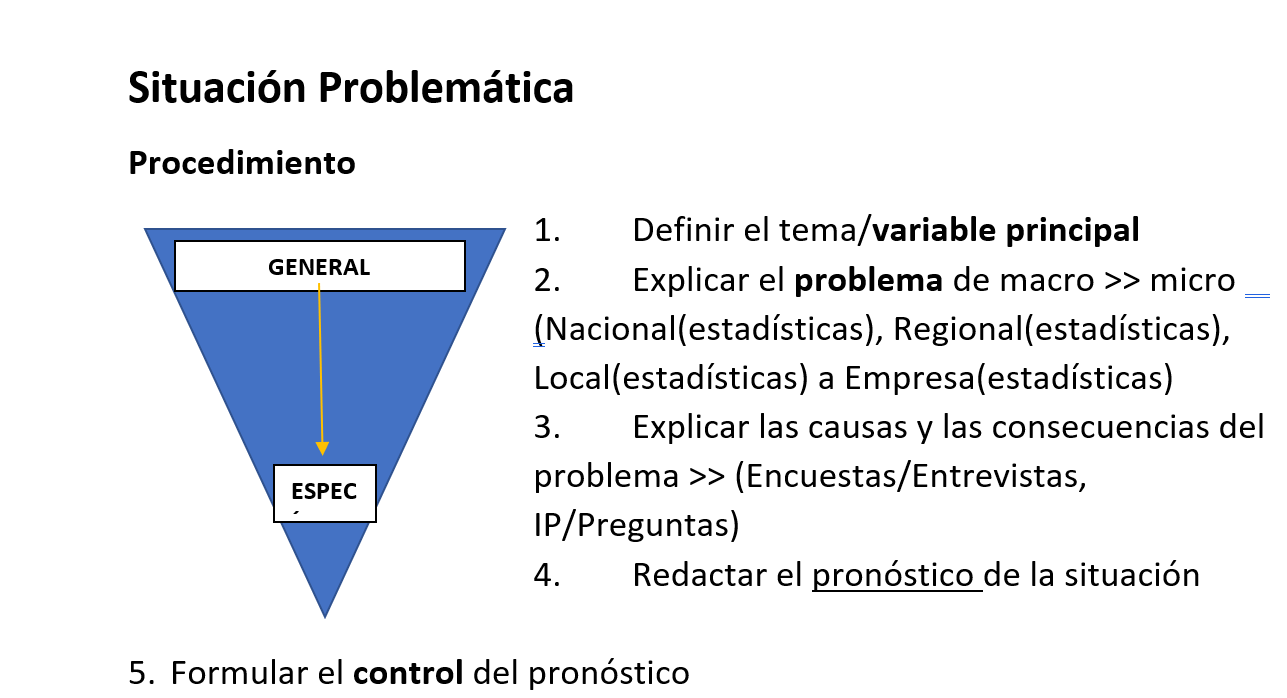
\includegraphics[scale=0.5]{img/problem_sec.png}

\section{Pregunta de Investigación}

La formulación de un problema consiste en la presentación oracional del mismo, es decir, “reducción del problema a términos concretos, explícitos, claros y precisos” (Tamayo, 1993), y es “la concreción del planteamiento en una pregunta precisa y delimitada en cuanto a espacio, tiempo y población (si fuere el caso)”. (Fidias G. Arias, 2006)

Debe cumplir:
\begin{itemize}
    \item Carecer de expresiones que implican juicios de valor: bueno, malo, mejor, etc.
    \item No originar respuestas tales como SI o No
    \item Estar delimitados en cuanto a tiempo y espacio y población
\end{itemize}

Puede ser de forma \textbf{Interrogativa/afirmativa}.


Por ejemplo:

Ejemplo 1:¿Cuál es el impacto de la satisfacción en la lealtad de los clientes en los restaurantes de comida china en Lima Metropolitana, 2019?

Ejemplo 2: ¿Cómo la alta rotación del personal incide en la productividad de la empresa Muebles Finos S.A.C. de la ciudad de Arequipa, 2019?

Ejemplo 3: ¿Cuáles son los factores que inciden en la motivación del personal de ventas de la empresa Jugos del Norte S.A. durante el periodo de 2018 y 2019?

\textbf{Elementos:}

\textbf{La interrogante:} es la pregunta clave que se planteará.

\textbf{Variable o variables:} la variable o variables que forman parte del estudio. En el caso de un estudio descriptivo será una variable, mientras que en un estudio correlacional serán dos variables.

\textbf{Enlace o relacionante:} el vínculo con el cual se relaciona las variables.

\textbf{Población:} es generalmente la colección de individuos u objetos que son el foco principal de la investigación científica, y que serán observados, encuestados o medidos.

\textbf{Delimitación espacial:} el lugar o zona geográfica que comprende el estudio. También comprende el ámbito específico de estudio, como por ejemplo puede ser una empresa determinada o conjunto de negocios (como los cinemas).

\textbf{Delimitación temporal:} el período de tiempo que comprende el estudio.




\chapter{Justificación}
\label{Justificación}

%Proyecto: Desarrollo de una Plataforma de Gestión de Proyectos Basada en la Nube}

\paragraph{Justificación Teórica}
La justificación teórica se refiere a la base conceptual y los principios científicos que sustentan el proyecto. Incluye: 

\begin{itemize}
    \item \textbf{Revisión de la literatura}: Se revisan estudios y publicaciones sobre gestión de proyectos, incluyendo metodologías ágiles como  Kanban, así como teorías sobre la colaboración en equipos distribuidos.
    \item \textbf{Fundamentos teóricos}: Se fundamenta en teorías de gestión de proyectos, colaboración en línea, y computación en la nube. Se citan trabajos de autores como Harold Kerzner en gestión de proyectos y estudios recientes sobre la eficacia de herramientas de colaboración en la nube.
    \item \textbf{Estado del arte}: Análisis de plataformas actuales de gestión de proyectos como Jira, Asana y Trello, identificando sus fortalezas y debilidades.
\end{itemize}
\textbf{Ejemplo de contenido}: "Las teorías de gestión de proyectos de Harold Kerzner (2017) subrayan la importancia de la planificación y la colaboración efectiva. Estudios recientes (Smith et al., 2020) muestran que las herramientas de gestión basadas en la nube pueden aumentar la eficiencia en equipos distribuidos en un 25\%."

\paragraph{Justificación Práctica}
La justificación práctica se enfoca en la utilidad y la aplicabilidad del proyecto. Se trata de demostrar la relevancia y la necesidad del proyecto en un contexto real. Incluye: 

\begin{itemize}
    \item \textbf{Problemas o necesidades}: Identificación de la necesidad de una plataforma que permita a los equipos distribuidos gestionar proyectos de manera más efectiva, con características específicas como la integración de comunicación en tiempo real y herramientas avanzadas de reporting.
    \item \textbf{Beneficios}: La plataforma propuesta permitirá una mayor eficiencia en la gestión de tareas, mejor comunicación entre los miembros del equipo y un seguimiento más preciso del progreso del proyecto. Esto reducirá los costos operativos y mejorará la productividad.
    \item \textbf{Aplicaciones}: Utilización en empresas de tecnología, agencias de marketing, y cualquier organización que trabaje con equipos distribuidos o gestione múltiples proyectos simultáneamente.
\end{itemize}
\textbf{Ejemplo de contenido}: "En una encuesta realizada por Project Management Institute (2019), el 60\% de las empresas informaron retrasos significativos en proyectos debido a la falta de herramientas de gestión adecuadas. Nuestra plataforma abordará esta necesidad proporcionando una solución integral que combina gestión de tareas, comunicación en tiempo real y reporting avanzado."

\paragraph{Justificación Metodológica}
La justificación metodológica describes los métodos y técnicas que se utilizaran para llevar cabo el proyecto. Incluye: 

\begin{itemize}
    \item \textbf{Métodos de investigación}: Uso de encuestas y entrevistas con potenciales usuarios para identificar características clave y requerimientos. Análisis de datos para entender las necesidades y preferencias de los usuarios.
    \item \textbf{Técnicas y herramientas}: Desarrollo ágil utilizando Scrum. Herramientas de desarrollo como React para el frontend, Node.js para el backend y servicios de AWS para la infraestructura en la nube.
    \item \textbf{Plan de trabajo}: El proyecto se dividirá en varias fases: investigación inicial (1 mes), diseño y planificación (2 meses), desarrollo (6 meses), pruebas (2 meses) y despliegue (1 mes). Cada fase incluirá iteraciones y revisiones periódicas con los stakeholders.
\end{itemize}
\textbf{Ejemplo de contenido}: "Utilizaremos la metodología Scrum para asegurar un desarrollo iterativo e incremental, con sprints de 2 semanas y revisiones periódicas. Las herramientas elegidas, como React y Node.js, permitirán una construcción rápida y flexible del frontend y backend, mientras que AWS proporcionará una infraestructura escalable y segura."

Este enfoque integral asegura que el proyecto esté bien fundamentado teóricamente, responda a necesidades prácticas reales y esté metodológicamente preparado para su desarrollo y éxito.

 

\chapter{Objetivos}
\label{Objetivos}

\subsubsection{Objetivo General}

\paragraph{¿Qué es?}

El objetivo general describe de manera amplia y comprensiva lo que se pretende alcanzar con el proyecto. Representa el propósito principal y la meta final del proyecto.

\paragraph{¿Cómo se elabora?}

\begin{enumerate}
    \item \textbf{Claridad}: Debe ser claro y comprensible. Evita el uso de términos ambiguos.
    \item \textbf{Amplitud}: Debe abarcar el alcance completo del proyecto.
    \item \textbf{Realismo}: Debe ser alcanzable y realista dentro del contexto y los recursos disponibles.
    \item \textbf{Redacción}: Generalmente se formula utilizando un verbo en infinitivo que indique una acción amplia, como "desarrollar", "mejorar", "crear", etc.
\end{enumerate}
\textbf{Ejemplo}: "Desarrollar una plataforma de gestión de proyectos basada en la nube para mejorar la colaboración y eficiencia en equipos distribuidos."

\subsubsection{Objetivos Específicos}

\paragraph{¿Qué son?}

Los objetivos específicos desglosan el objetivo general en metas más concretas y detalladas. Cada objetivo específico aborda un aspecto particular del proyecto y contribuye al logro del objetivo general.

\paragraph{¿Cómo se elaboran?}

\begin{enumerate}
    \item \textbf{Desglose}: Identifica las principales etapas, componentes o aspectos del proyecto necesarios para alcanzar el objetivo general.
    \item \textbf{Precisión}: Deben ser específicos y detallados, describiendo claramente qué se va a hacer.
    \item \textbf{Medibilidad}: Siempre que sea posible, deben ser medibles para evaluar el progreso y el éxito.
    \item \textbf{Redacción}: También se formulan utilizando verbos en infinitivo que indiquen acciones concretas, como "diseñar", "implementar", "evaluar", etc.
\end{enumerate}
\textbf{Ejemplo}:

\begin{enumerate}
    \item "Diseñar la interfaz de usuario de la plataforma para asegurar una experiencia intuitiva y amigable para los usuarios."
    \item "Implementar funciones de comunicación en tiempo real para facilitar la colaboración entre miembros del equipo."
    \item "Desarrollar herramientas de reporting avanzado para proporcionar seguimiento detallado del progreso de los proyectos."
    \item "Realizar pruebas de usabilidad para identificar y corregir posibles problemas antes del lanzamiento."
    \item "Implementar medidas de seguridad en la plataforma para proteger los datos de los usuarios y la integridad del sistema."
\end{enumerate}

\subsubsection{Pasos para Redactar los Objetivos}

\begin{enumerate}
    \item \textbf{Identifica el propósito del proyecto}: Reflexiona sobre el problema que deseas resolver o la mejora que quieres lograr.
    \item \textbf{Define el objetivo general}: En una oración clara, describe el resultado principal que esperas alcanzar.
    \item \textbf{Desglosa en objetivos específicos}: Divide el objetivo general en varias metas más pequeñas y detalladas, asegurando que cada una sea una parte integral del logro del objetivo general.
    \item \textbf{Verifica coherencia y factibilidad}: Asegúrate de que todos los objetivos específicos sean coherentes entre sí y con el objetivo general, y que sean alcanzables con los recursos y el tiempo disponibles.
    \item \textbf{Redacción final}: Redacta cada objetivo de manera clara y precisa, utilizando verbos en infinitivo para indicar acción.
\end{enumerate}

\subsubsection{Ejemplo Completo:}

\textbf{Objetivo General}: "Desarrollar una plataforma de gestión de proyectos basada en la nube para mejorar la colaboración y eficiencia en equipos distribuidos."

\textbf{Objetivos Específicos}:

\begin{enumerate}
    \item "Diseñar la interfaz de usuario de la plataforma para asegurar una experiencia intuitiva y amigable para los usuarios."
    \item "Implementar funciones de comunicación en tiempo real para facilitar la colaboración entre miembros del equipo."
    \item "Desarrollar herramientas de reporting avanzado para proporcionar seguimiento detallado del progreso de los proyectos."
    \item "Realizar pruebas de usabilidad para identificar y corregir posibles problemas antes del lanzamiento."
    \item "Implementar medidas de seguridad en la plataforma para proteger los datos de los usuarios y la integridad del sistema."
\end{enumerate}
Este enfoque asegura que el proyecto esté bien orientado y que cada fase y tarea esté claramente definida, lo que facilita su gestión y ejecución exitosa.

 


%\chapter{Alcance}
\label{Alcance}



\chapter{Marco Teórico}
\label{MarcoTeorico}
\chapter{Metodología}
% Please add the following required packages to your document preamble:
% \usepackage{graphicx}
\begin{table}[]
\caption{Metodología del PTT}
\label{tab:metodologia}
\resizebox{\textwidth}{!}{%
\begin{tabular}{|l|l|l|l|l|l|l|}
\hline
\multicolumn{1}{|c|}{\textbf{OBJETIVOS}} &
  \multicolumn{1}{c|}{\textbf{ALCANCE}} &
  \multicolumn{1}{c|}{\textbf{RESULTADO}} &
  \multicolumn{1}{c|}{\textbf{MÉTODOS/TEC}} &
  \multicolumn{1}{c|}{\textbf{MATERIALES}} &
  \multicolumn{1}{c|}{\textbf{LUGAR}} &
  \multicolumn{1}{c|}{\textbf{RESPONSABLE}} \\ \hline
\textbf{OB1 \ref{OB1}} &
   &
  Modelo de BPM &
  \begin{tabular}[c]{@{}l@{}}RAD:BPM\\ BPM\end{tabular} &
   &
  \begin{tabular}[c]{@{}l@{}}CIS\\ UNL\end{tabular} &
  Diana y Cesar \\ \hline
\textbf{OB2} &
  \begin{tabular}[c]{@{}l@{}}AC1\\ AC2\\ AC3\end{tabular} &
  Prototipo de Software &
  XP &
  \begin{tabular}[c]{@{}l@{}}Historias de Usuario\\ Diagrama de Clases\\ Python, Django\\ Postglres\end{tabular} &
  lab de software &
  \begin{tabular}[c]{@{}l@{}}Diana \\ Cesar\\ Diana y Cesar\end{tabular} \\ \hline
\textbf{OB3} &
   &
  \begin{tabular}[c]{@{}l@{}}Estadística de validación\\ Informe técnico\\ Artículo técnico\end{tabular} &
  \begin{tabular}[c]{@{}l@{}}Análisis C.\\ Prueba de H\end{tabular} &
   &
   &
   \\ \hline
\end{tabular}%
}
\end{table}
\chapter{Cronograma}
\label{Cronograma}
Para mas información revisar \cite{gantt}
\import{Secciones/}{7_Cronograma}
\chapter{Presupuesto y Financiamiento}
\label{Presupuesto}
 
\bibliographystyle{ieeetr}%Used BibTeX style
\bibliography{Config/bib}

%%%%
% CONTENIDO. LISTA DE ACRÓNIMOS. Comenta las líneas si no lo deseas incluir.
%%%%
% Incluye el listado de acrónimos utilizados en el trabajo. 
\printglossary[style=modsuper,type=\acronymtype,title={Lista de Acrónimos y Abreviaturas}]
% Añade el resto de acrónimos si así se desea. Si no elimina el comando siguiente
\glsaddallunused 

%%%%
% CONTENIDO. Anexos - Añade o elimina según tus necesidades
%%%%
\appendix % Inicio de los apéndices
%%%%%%%%%%%%%%%%%%%%%%%%%%%%%%%%%%%%%%%%%%%%%%%%%%%%%%%%%%%%%%%%%%%%%%%%
% Plantilla TFG/TFM
% Escuela Politécnica Superior de la Universidad de Alicante
% Realizado por: Jose Manuel Requena Plens
% Contacto: info@jmrplens.com / Telegram:@jmrplens
%%%%%%%%%%%%%%%%%%%%%%%%%%%%%%%%%%%%%%%%%%%%%%%%%%%%%%%%%%%%%%%%%%%%%%%%


% Ejemplo de páginas en horizontal y vertical

\chapter{Páginas horizontales}
Aquí se muestra cómo incluir páginas en horizontal.

Esta página está en vertical\\
\clearpage % Nueva página

\begin{landscape} % Inicia modo horizontal
	

Esta página está en horizontal\\
\clearpage % Nueva página

Esta página también está en horizontal\\

\end{landscape} % Finaliza modo horizontal
\clearpage % Nueva página


Esta página está de nuevo en vertical\\




%%%%%%%%%%%%%%%%%%%%%%%%%%%%%%%%%%%%%%%%%%%%%%%%%%%%%%%%%%%%%%%%%%%%%%%%
% Plantilla TFG/TFM
% Escuela Politécnica Superior de la Universidad de Alicante
% Realizado por: Jose Manuel Requena Plens
% Contacto: info@jmrplens.com / Telegram:@jmrplens
%%%%%%%%%%%%%%%%%%%%%%%%%%%%%%%%%%%%%%%%%%%%%%%%%%%%%%%%%%%%%%%%%%%%%%%%

% Ejemplo de inclusión de páginas de un PDF

\chapter{Importar PDF}

A continuación se muestra una página importada de un PDF externo. Observar los comentarios en el código de este anexo para más información. También puedes leer el manual con todas las opciones en \url{http://osl.ugr.es/CTAN/macros/latex/contrib/pdfpages/pdfpages.pdf}.

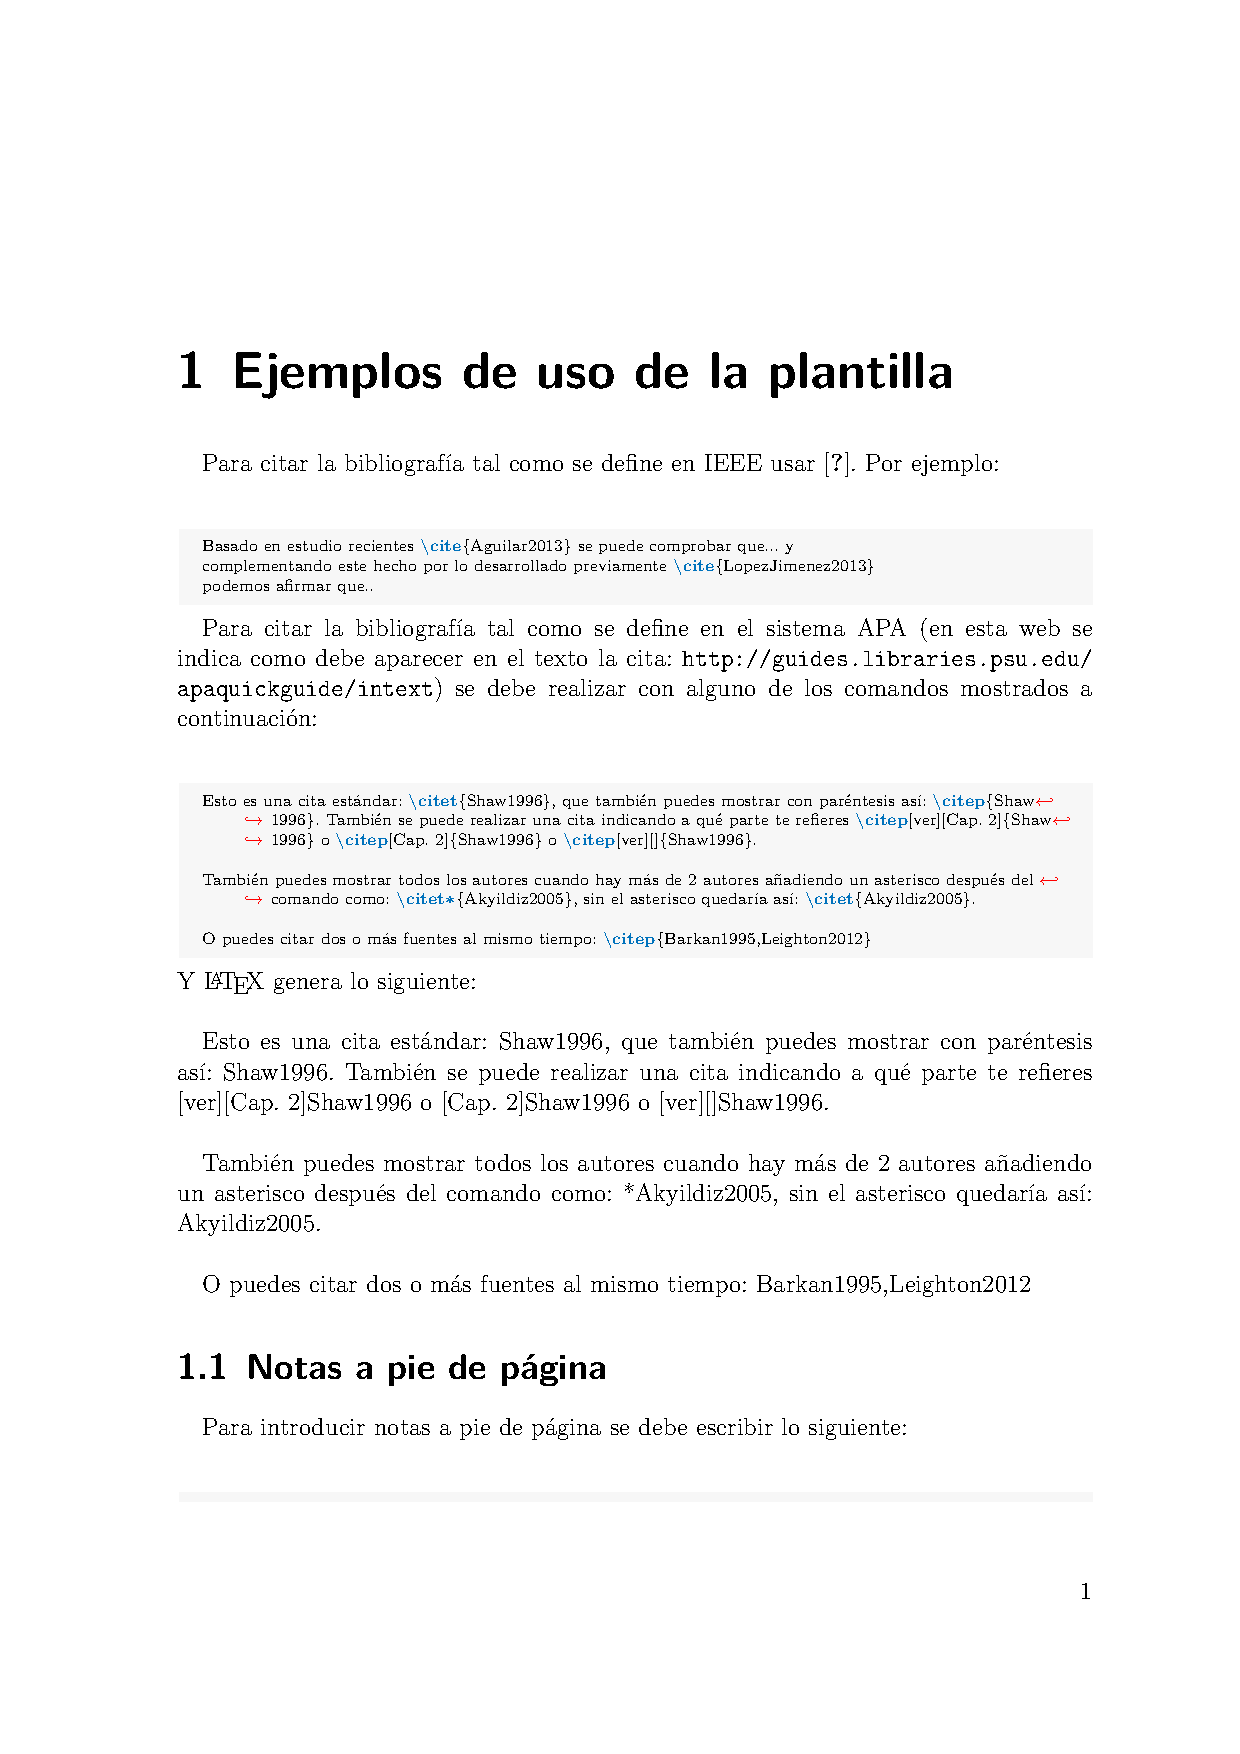
\includepdf[pages=-]{Anexos/ejemplos.pdf}

% Para incluir una página:
% [pages={0}] % Donde '0' es el número de la pagina del PDF que se quiere incluir

% Para incluir varias páginas consecutivas
% [pages={1-4}] % Con estos valores importa de la página 1 a la 4.

% Para incluir varias páginas salteadas
% [pages={1,4,7,10}] % Incluye las páginas 1,4,7 y 10

% Para incluir todo el documento PDF
% [pages=-]

% Si ademas de pages=... se incluye landscape, se importa en horizontal
% [pages{1},landscape]
%%%%%%%%%%%%%%%%%%%%%%%%%%%%%%%%%%%%%%%%%%%%%%%%%%%%%%%%%%%%%%%%%%%%%%%%
% Plantilla TFG/TFM
% Escuela Politécnica Superior de la Universidad de Alicante
% Realizado por: Jose Manuel Requena Plens
% Contacto: info@jmrplens.com / Telegram:@jmrplens
%%%%%%%%%%%%%%%%%%%%%%%%%%%%%%%%%%%%%%%%%%%%%%%%%%%%%%%%%%%%%%%%%%%%%%%%

\chapter{Anexo I}
Aquí el anexo...



\end{document}